\chapter{Actions of Groups}

\section{Group Actions}

\begin{definition}[Action]\index{action (of a group)}\label{def:action}
    Let $G$ be a group and $X$ a set. We say $G$ \term{acts on $X$} if there is a map \[
        \begin{matrix}[rccc]
            \cdot: & G \times X & \to     & X \\
                   & (g, x)     & \mapsto & g \cdot x
        \end{matrix}
    \] such that \begin{enumerate}
        \item $e \cdot x = x$ for all $x \in X$.
        \item $g \cdot (h \cdot x) = (g \cdot h) \cdot x$ for all $g, h \in G$ and $x \in X$.
    \end{enumerate}
\end{definition}

Associated with an action, there are three important constructions.

\begin{definition}[Orbit]\index{orbit}\label{def:orbit}
    Let $G$ act on $X$. The \term{orbit} of $x \in X$ is the set \[
        \mathcal{O}_x = \{ g \cdot x \mid g \in G \}.
    \]
\end{definition}

\begin{definition}[Stabilizer]\index{stabilizer}\label{def:stabilizer}
    Let $G$ act on $X$. The \term{stabilizer} of $x \in X$ is the set \[
        Stab_x(G) = \{ g \in G \mid g \cdot x = x \}.
    \]
\end{definition}

We can think of a group action as a homomorphism from $G$ to group of bijections of $X$, \[
    G \xrightarrow{\varphi} \sum (X) = \{ f: X \to X \mid f \text{ is a bijection} \}.
\]

\begin{example}
    Given a group $G$ we say $G$ acts on itself by conjugation by defining \[
        h^g = C_g(h) = g h g^{-1}.
    \] This is an action. 
    \begin{listu}
        \item $1 \cdot x = 1 \cdot x \cdot 1^{-1} = x$
        \item $C_(C_h(k)) = C_g(hkh^{-1}) = ghkh^{-1}g^{-1} = ghk(gh)^{-1} = (gh) \cdot k = C_{gh}(k)$
    \end{listu}
\end{example}

\begin{definition}[Conjugacy Class]\index{conjugacy class}\label{def:conjugacy-class}
    The orbit under conjugation is called the \term{conjugacy class} of $G$.
\end{definition}

\begin{remark}
    Conjugacy classes is \bred{not a subgroup} of $G$.
\end{remark}

\begin{example}
    Consider $S_3 = \{ e, (12), (13), (23), (123), (132) \}$.

    \begin{minipage}[t]{0.45\linewidth} \begin{listu}
        \item $(12) 1 (12)^{-1} = 1$
        \item $(12) (12) (12)^{-1} = (12)$
        \item $(12) (13) (12)^{-1} = (23)$
        \item $(12) (23) (12)^{-1} = (13)$
        \item $(12) (123) (12)^{-1} = (132)$
        \item $(12) (132) (12)^{-1} = (123)$
    \end{listu} \end{minipage}
    \begin{minipage}[t]{0.45\linewidth} \begin{listu}
        \item $(123) 1 (123)^{-1} = 1$
        \item $(123) (12) (123)^{-1} = (23)$
        \item $(123) (13) (123)^{-1} = (12)$
        \item $(123) (23) (123)^{-1} = (13)$
        \item $(123) (123) (123)^{-1} = (123)$
        \item $(123) (132) (123)^{-1} = (132)$
    \end{listu} \end{minipage}
\end{example}

\begin{example}
    Now consider $S_4$. 

    \begin{minipage}[t]{0.45\linewidth} \begin{listu}
        \item $(12) 1 (12)^{-1} = 1$
        \item $(12) (12) (12)^{-1} = (12)$
        \item $(12) (13) (12)^{-1} = (23)$
        \item $(12) (14) (12)^{-1} = (24)$
        \item $(12) (23) (12)^{-1} = (13)$
        \item $(12) (24) (12)^{-1} = (14)$
    \end{listu} \end{minipage}
    \begin{minipage}[t]{0.45\linewidth} \begin{listu}
        \item $(12) (34) (12)^{-1} = (34)$
        \item $(12) (12)(34) (12)^{-1} = (12)(34)$
        \item $(12) (13)(24) (12)^{-1} = (14)(23)$
        \item $(12) (14)(23) (12)^{-1} = (13)(24)$
        \item $\cdots$
    \end{listu} \end{minipage}

    We can see that in both examples, the cycle structure is preserved under conjugation. This brings to a very important theorem.
\end{example}

\begin{theorem}
    The conjugacy classes of $S_n$ are classified by the cycle structure of the elements.
\end{theorem}

\begin{example}
    Consider $S_4$, it has the following cycle structures: \[
        (a)(b)(c)(d), \quad (ab), \quad (ab)(cd), \quad (abc), \quad (abcd);
    \] which has \[
        1, \quad 6, \quad 3, \quad 8, \quad 6
    \] elements, respectively.
\end{example}

\begin{example}
    Let $G$ be the set of $n \times n$ matrices over $\C$.

    If $\begin{pmatrix} a & b \\ c & d \end{pmatrix}$ is such a $2 \times 2$ matrix that is diagonalizable, then that means there is a basis of eigenvectors $\{ v_1, v_2 \}$.

    Then, \[
        \begin{pmatrix} a & b \\ c & d \end{pmatrix} = Q \begin{pmatrix} \lambda_1 & 0 \\ 0 & \lambda_2 \end{pmatrix} Q^{-1}.
    \] where $Q$ is the change of basis matrix from the standard basis to the basis of eigenvectors.

    That is, \[
        Q = (v_1, v_2) = \begin{pmatrix} v_{11} & v_{12} \\ v_{21} & v_{22} \end{pmatrix}.
    \]

    We see in generalized eigenvectors that we can either conjugate the matrix to Jordan form $\begin{pmatrix} \lambda & 1 \\ 0 & \lambda \end{pmatrix}$, or we can conjugate the matrix to a block diagonal matrix $\begin{pmatrix} \lambda_1 & 0 \\ 0 & \lambda_2 \end{pmatrix}$.

    Consider if we want to answer if $\begin{pmatrix} 1 & 7 \\ 2 & 3 \end{pmatrix}$ and $\begin{pmatrix} 7 & 5 \\ 1 & i \end{pmatrix}$ conjugate, that is, if there exists a matrix $Q$ such that \[
        \begin{pmatrix} 1 & 7 \\ 2 & 3 \end{pmatrix} = Q \begin{pmatrix} 7 & 5 \\ 1 & i \end{pmatrix} Q^{-1}.
    \]

    A na\"ive approach would be to solve for the eigenvalues of the two matrices, and then solve for the eigenvectors; however, this is not the most efficient way, as calculating the eigenvalues of a matrix is a difficult problem.

    We see that the determinant is preserved under conjugation, so the two matrices are not conjugate.

    Now consider $\begin{pmatrix} 1 & 7 \\ 3 & 2 \end{pmatrix}$ and $\begin{pmatrix} 1 & 2 \\ 0 & -19 \end{pmatrix}$. They have the same determinant, but are they conjugate?

    The answer is no. We need the trace to be preserved as well.

    This is because the determinant and the trace are all operations on the eigenvalues of the matrix (the determinant is the product of the eigenvalues, and the trace is the sum), and the eigenvalues are preserved under conjugation.

    \begin{remark}[Characteristic Polynomial]\index{Characteristic Polynomial}
        Consider an $n \times n$ matrix $A$. The characteristic polynomial of $A$, denoted by $p_A(t)$, is the polynomial defined by \[
            p_A(t) = \det{(tI - A)}.
        \] where $I$ denotes the $n \times n$ identity matrix.
    \end{remark}

    Thus, we need to check the characteristic polynomial of the two matrices to see if they are conjugate. The coefficients of the characteristic polynomial are precisely the invariants of the matrix under conjugation.

    The conjugacy classes is a replacement of eigenvalues. 
\end{example}

\section{Orbit-Stabilizer Theorem}

\begin{theorem}[Cauchy's Theorem]\index{Cauchy's Theorem}\label{thm:cauchy}
    Let $G$ be a finite group and $p$ be a prime number. If $p$ divides the order of $G$, then there exists an element $x \in G$ of order $p$.
\end{theorem}

\begin{example}
    Let $n = 15$, and $|D_{15}| = 30 = 2 \cdot 3 \cdot 5$.

    Then, by Cauchy's Theorem, there exists an element of order $2$, $3$, and $5$ in $D_{15}$.
\end{example}

\begin{example}
    Consider $S_7$. We have $|S_7| = 7! = 2^4 \cdot 3^2 \cdot 5 \cdot 7$.

    Then, by Cauchy's Theorem, there exists an element of order $2$, $3$, $5$, and $7$ in $S_7$.
\end{example}

\begin{example}
    Consider $\RR$. We have $|\RR| = 48 = 2^4 \cdot 3$.

    Then, by Cauchy's Theorem, there exists an element of order $2$ and $3$ in $\RR$.
\end{example}

{~~~}

There are two observations to make about conjugation,
\begin{listu}
    \item If $x \in G$ is fixed by the conjugation, that is, $gxg^{-1} = x$ for all $g \in G$, then $x$ is in the center of $G$.

    \item All conjugacy classes are disjoint. 
\end{listu}

\begin{figure}[ht!]
    \centering
    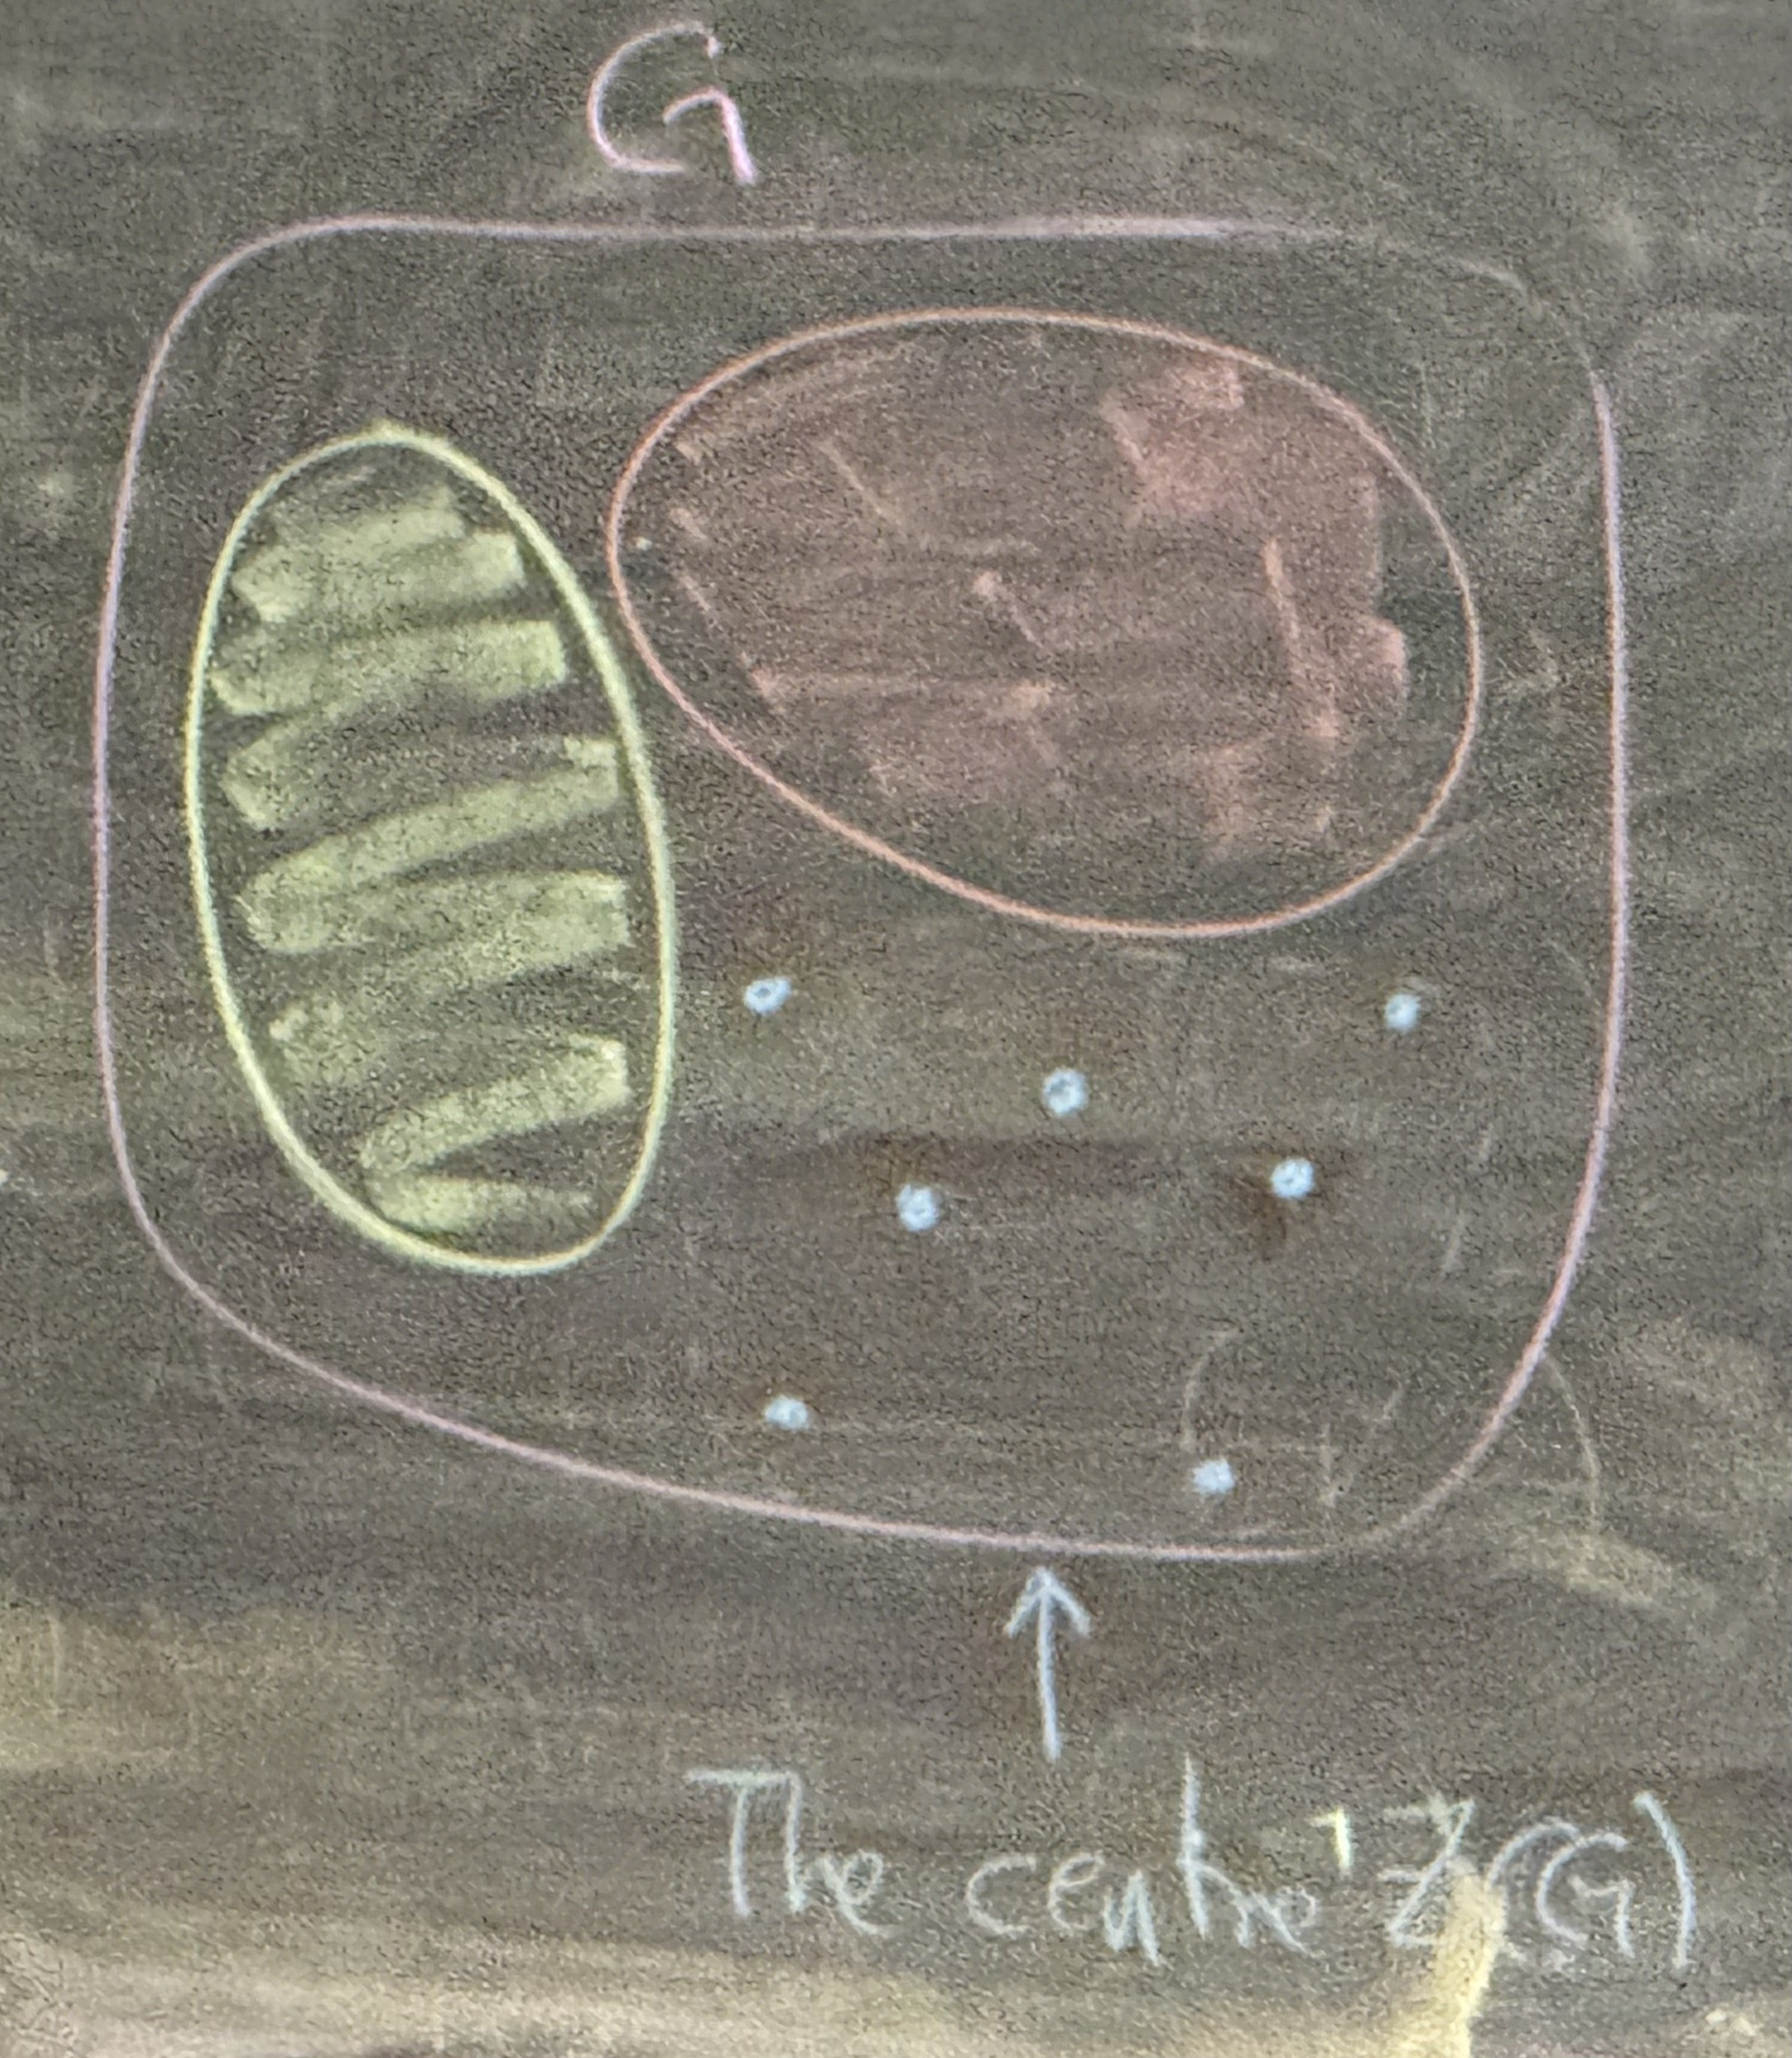
\includegraphics[width=0.2\linewidth]{figures/conjugacy-class.jpg}
\end{figure}

From this we get \[
        |G| = |Z(G)| + \sum_{\substack{x \notin Z(G) \\\text{without repeating conjugacy classes}}} | Conj(x) |.
\] This equation is called the \term{class equation}\index{class equation}.

\begin{theorem}[Orbit-Stabilizer Theorem]\index{orbit-stabilizer theorem}\label{thm:orbit-stabilizer}
    Let $G$ be a finite group acting on a set $X$. Then, for any $x \in X$, \[
        | G | =  | \mathcal{O}_x | \cdot | Stab_x(G) |.
    \]

    It can also be written as \[
        G / Stab_x(G) \cong \mathcal{O}_x.
    \]
\end{theorem}

\begin{listu}
    \item $\mathcal{O}_x$ are all elements of $X$ I can reach from $x$. 
    \item $Stab_x(G)$ are all elements of $G$ that fix $x$ (i.e. $g \cdot x = x$).
\end{listu}

\begin{proof}
    Let $x \in X$ and $\mathcal{O}_x = \{ h \cdot x \mid g \in G \} = \{ x_1, x_2, \dots, x_k \}$.

    We make a table \begin{table}[ht!]
        \centering
        \begin{tabular}{c|c}
                      & Elements $g$  s.t. $g \cdot x = x_i$                       \\ \hline
            $x = x_1$ & $g \cdot x = x$ I have written the elements of $Stab_x(G)$ \\ \hline
            $x_2$     & $g \cdot x = x_2$                                          \\ \hline
            $\vdots$  & $\vdots$                                                   \\ \hline
            $x_k$     & $g \cdot x = x_k$
        \end{tabular}
    \end{table}
    % \begin{figure}[ht!]
        % \centering
    \begin{center}
        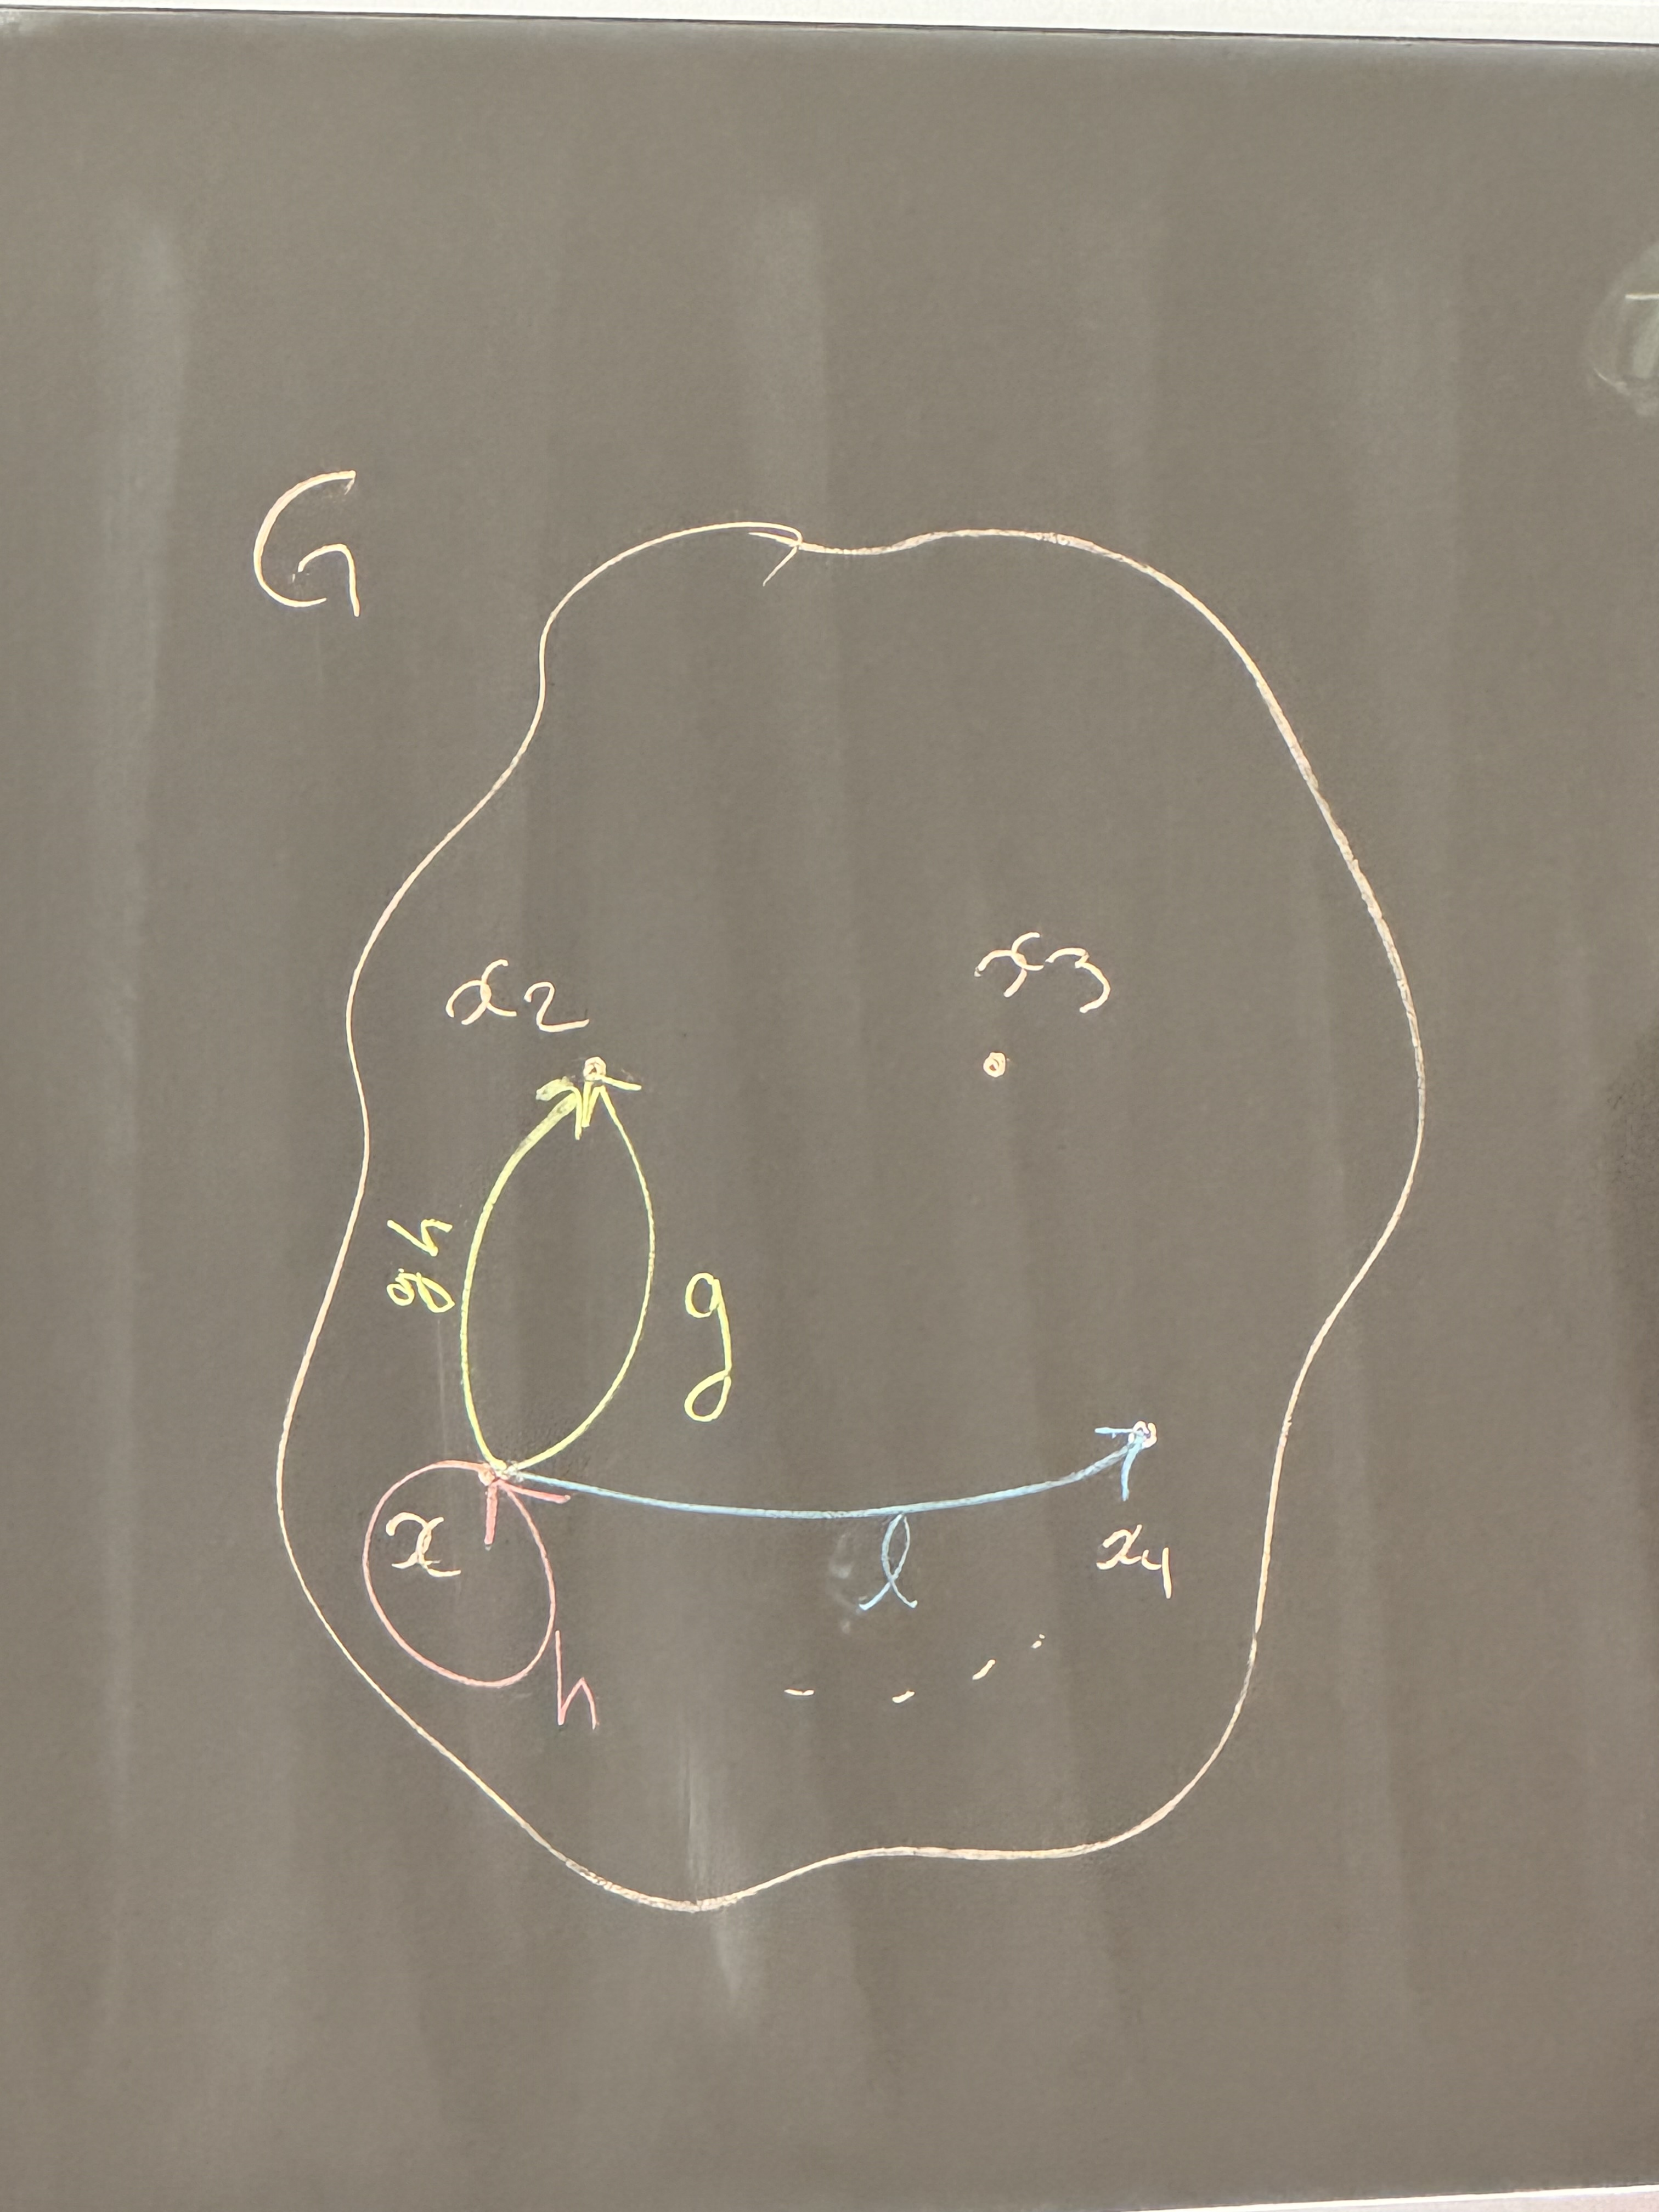
\includegraphics[width=0.2\linewidth]{figures/orbit-stabilizer-proof.jpg}
    % \end{figure}
    \end{center}

    We can write \[
        gh
    \] with $h \in Stab_x(G)$ and $g \cdot x = x_2$ and get \[
        gx \cdot x = g \cdot (h \cdot x) = g \cdot x = x_2
    \]

    With this we see that $g Stab_x(G)$ satisfies to only one element of $\mathcal{O}_x$. This is a coset of $Stab_x(G)$.

    % \begin{table}[ht!]
    %     \centering
    %     \begin{tabular}{c|c}
    %                   & Elements $g$  s.t. $g \cdot x = x_i$                       \\ \hline
    %         $x = x_1$ & $g \cdot x = x$ I have written the elements of $Stab_x(G)$ \\ \hline
    %         $x_2$     & $g \cdot x = x_2$                                          \\ \hline
    %         $\vdots$  & $\vdots$                                                   \\ \hline
    %         $x_k$     & $g \cdot x = x_k$
    %     \end{tabular}
    % \end{table}

    However, there may be an $x_i$ who produces more than one cosets, so we cannot make the claim yet.

    % \begin{figure}[ht!]
        % \centering
    \begin{center}
        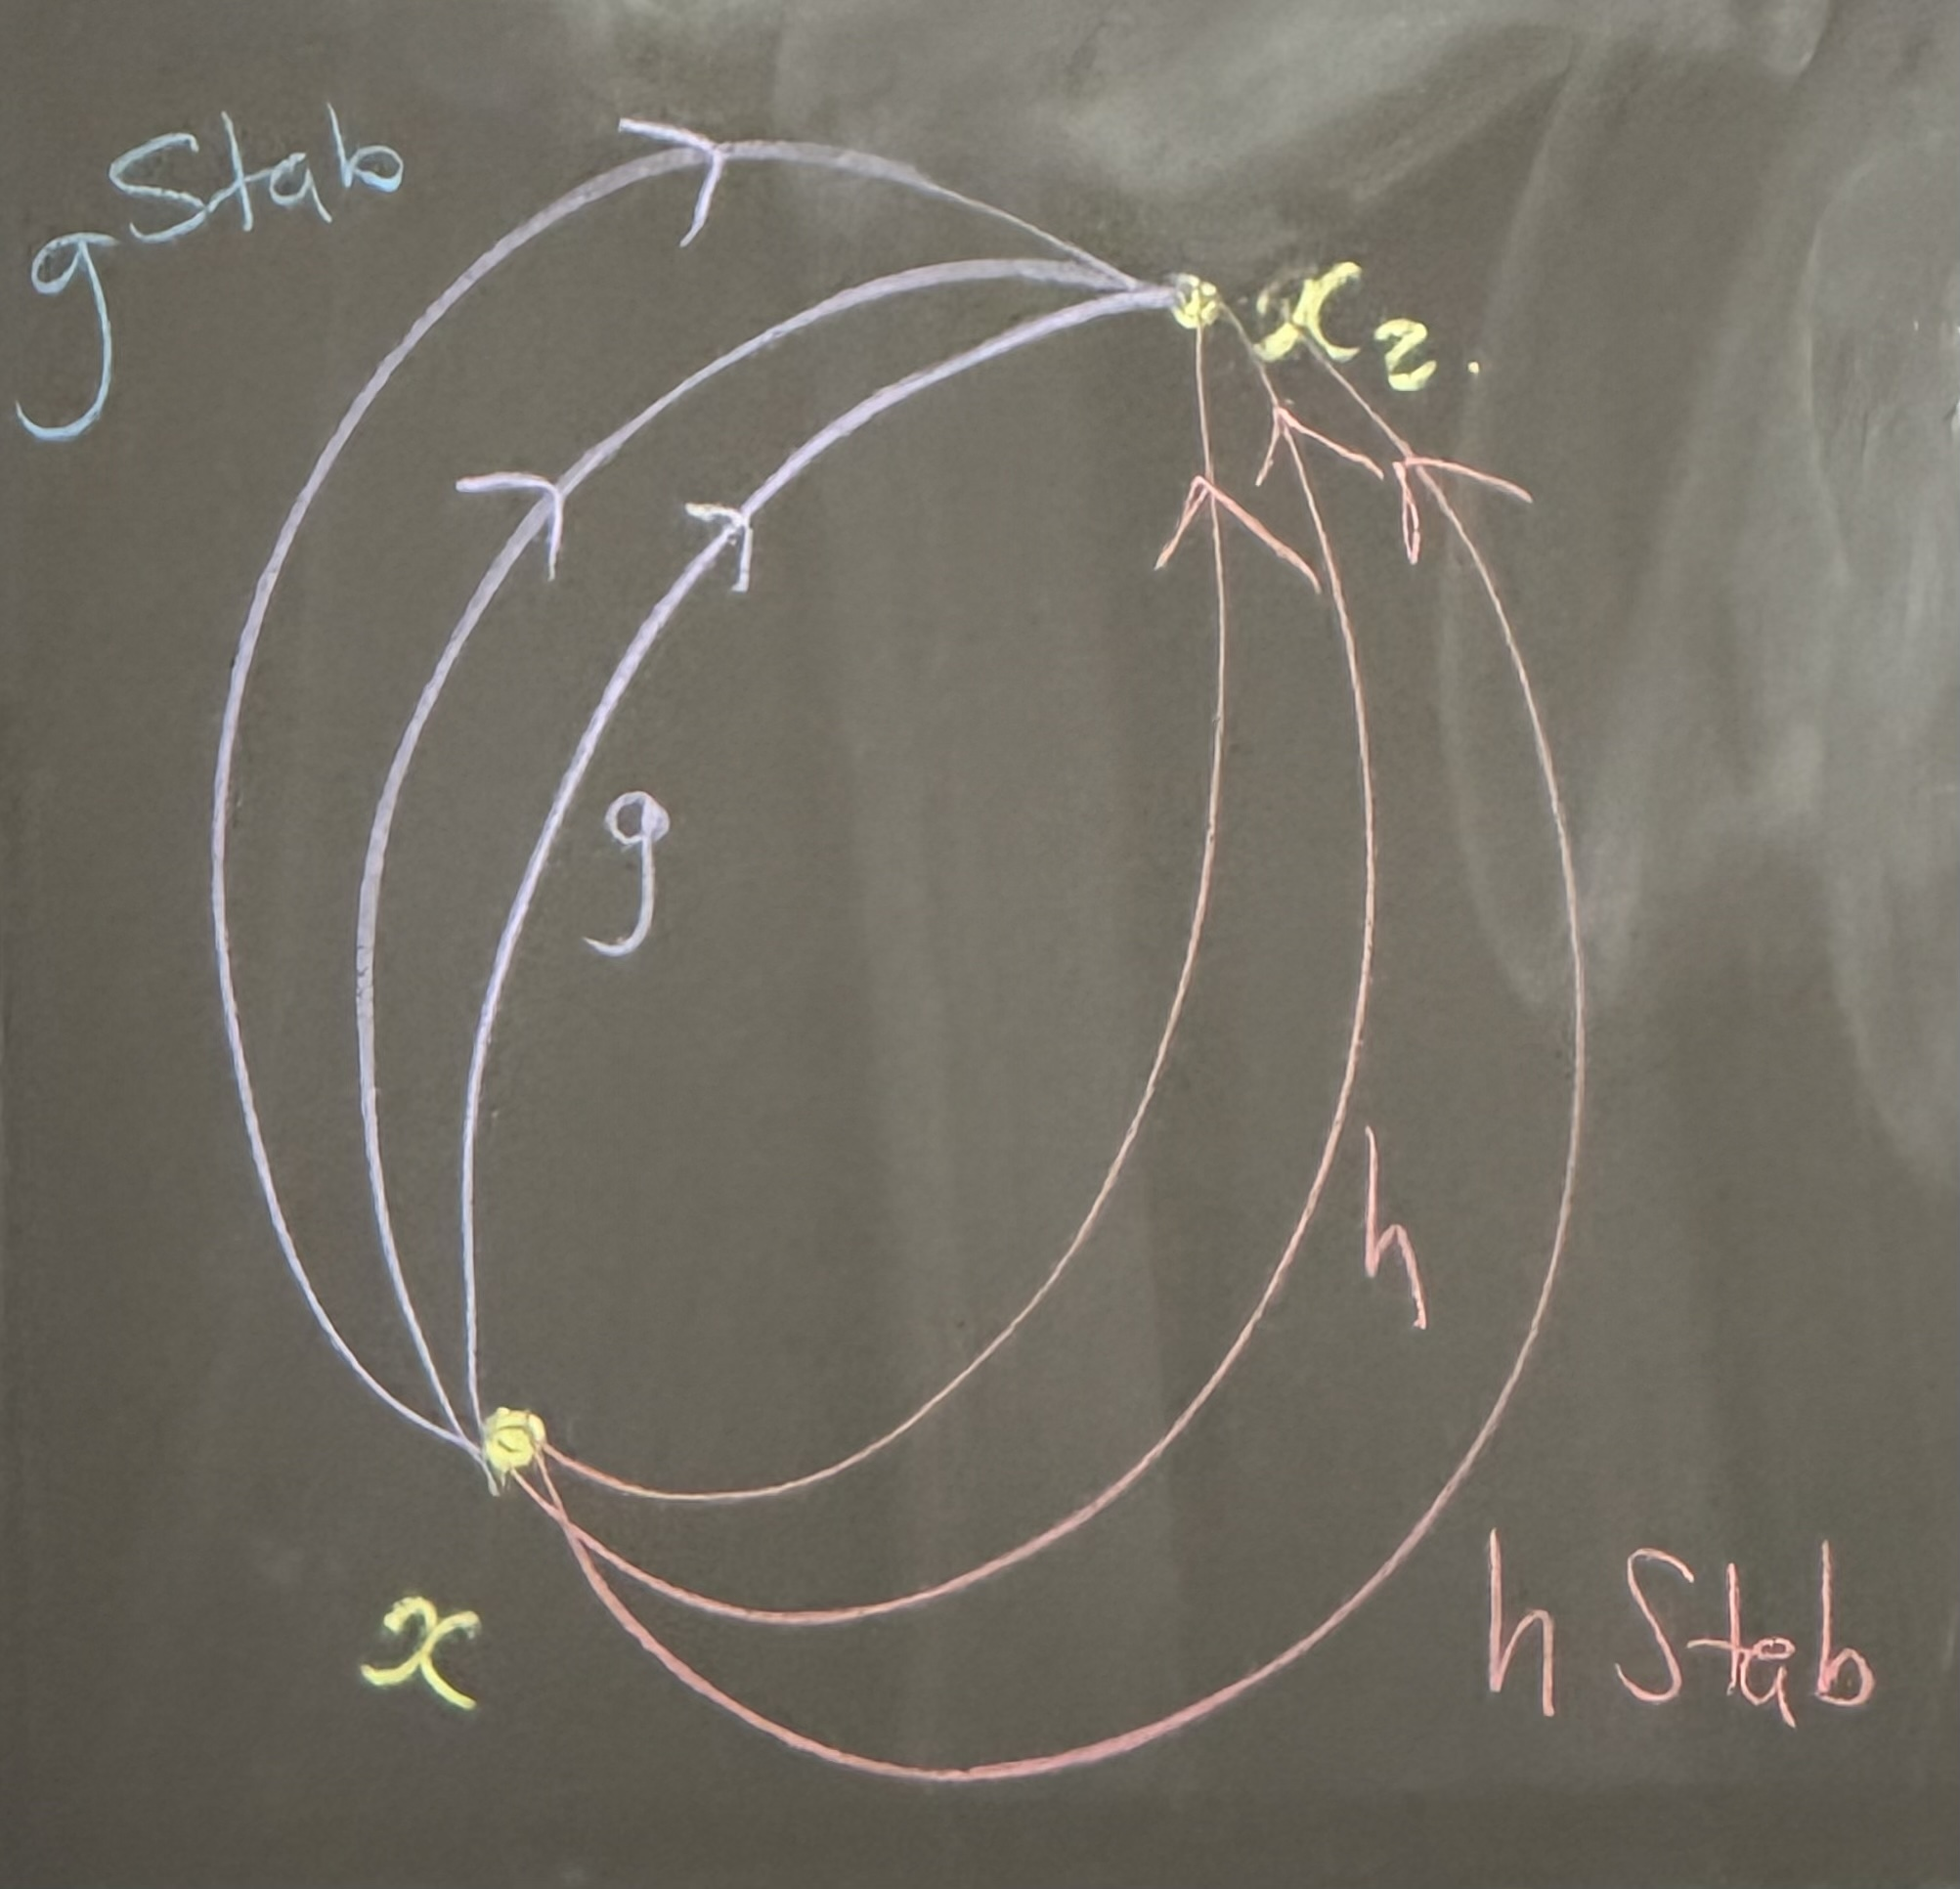
\includegraphics[width=0.2\linewidth]{figures/orbit-stabilizer-proof-2.jpg}
    \end{center}
    % \end{figure}

    If a row contains $g$ and $h$, then they must be in the same coset of $Stab_x(G)$.

    Indeed, $g^{-1} \cdot (h \cdot x) = g^{-1} \cdot x_2 = x$, thus $g^{-1} h \in Stab_x(G)$.

    This is the criteria for two elements to be in the same coset. Thus $g$ and $h$ are in the same coset.
    % We consider the path $x \overrightarrow{g} x_2 \overrightarrow{h} x$. 

    Then $|G| = \underset{Number of rows}{| \mathcal{O}_x |} \cdot \underset{Number of elements in each row}{| Stab_x(G) |}$.
\end{proof}

\begin{example}
    Consider the proof for \hyperref[thm:cauchy]{Cauchy's Theorem}.

    \begin{proof}
        Suppose we know the result for two cases:

        \begin{listo}
            \item If $H$ is abelian
            \item If $|H| < |G|$
        \end{listo}

        Let us use the class equation \[
            |G| = |Z(G)| + \sum_{\substack{x \notin Z(G) \\\text{without repeating conjugacy classes}}} | Conj(x) |.
        \]

        We know $p \mid |G|$. We have two possibilities: \begin{enumerate}
            \item $p \mid |Z(G)|$

            In this case, we are done.

            \item $p \not\mid |Z(G)|$

            We consider the conjugacy classes. 

            Known that $|G| = |Conj(x)| \cdot |Stab_x(G)|$ by the \hyperref[thm:orbit-stabilizer]{Orbit-Stabilizer Theorem}, and $|Stab_x(G)| < |G|$, so we fall under the second case ($|H| < |G|$).

            The only case remaining is if $p \mid |Conj(G)|$ and $p \not\mid |Z(G)|$.

            However, this is not possible, as $|Conj(G)| = |G| - |Z(G)|$, and $p \not\mid |Z(G)|$. 
        \end{enumerate}
    \end{proof}
\end{example}

\section{Sylow Theorems}

\subsection{First Sylow Theorem}

\begin{definition}[p-Group]\index{p-Group}\label{def:p-group}
    If $G$ is a group and $p \mid |G|$ for some prime $p$, then we say $H \leq G$ is a \term{p-group} if $|H| = p^k$ for some $k \geq 0$.
\end{definition}

\begin{example}
    If $|G| = 20$ and $H$ is a $2$-group of $G$, then $k \le 2$. 

    When $k = 0$, $|H| = 1$, and when $k = 1$, $|H| = 2$.
\end{example}

\begin{definition}[p-Sylow Subgroup]\index{p-Sylow subgroup}\label{def:p-sylow-subgroup}
    Let $G$ be a group and $p$ be a prime number. A \term{p-Sylow subgroup} of $G$ is a subgroup $H \leq G$ such that \begin{enumerate}
        \item $|H| = p^k$ for some $k \geq 0$ (i.e. $H$ is a p-group).
        % \item $p \nmid |G / H|$.
        \item For all p-groups $N$ of $G$, we cannot have $H \lneq N$ ($H \leq N$ and $H \neq N$) \footnote{A p-Sylow group cannot be strictly inside another p-group.}.
        
        In other words, a p-Sylow subgroup is a maximal p-group.
    \end{enumerate}
\end{definition}

\begin{example}
    Consider $G = \Z / n \Z$. We have $|G| = n$.

    Notice that the group generated by $n / p^a \in G$ has size $p^a$.
    
    This is a p-Sylow subgroup of $G$.
\end{example}

\begin{example}
    In $S_3$ the we have 
    \begin{itemize}
        \item $2$-groups $\{ 1, (12) \}$, $\{ 1, (13) \}$, and $\{ 1, (23) \}$
        \item $2$-Sylow subgroup $\{ 1, (123), (132) \}$
    \end{itemize}
\end{example}

\begin{theorem}[The First Sylow Theorem]\index{First Sylow Theorem}\label{thm:first-sylow}
    If $|G| = p^{a} \cdot m$ where $p \not\mid m$, then any $p$-Sylo group has size $p^a$. 
\end{theorem}

\begin{proof}
    Consider the collection $X = \{ A \subset G \mid |A| = p^a \}$.

    Consider the action \[ \begin{matrix}
        G \times X & \to & X \\
        (g, A)    & \mapsto & \{ g \cdot a, a \in A \}
    \end{matrix} \]

    We want to find an element $A \in X$ such that $|Stab_G(A)| = p^a$.

    We want to use the orbit stabilizer theorem to show that necessarily there is such collection $A$. \[
        |G| = | G \cdot A | \cdot | Stab_G(A) |.
    \]

    We have to show that there is an $A$ such that $|G \cdot A| = m$.

    Because $G \times X \to X$ is an action and orbits from a partition of $X$, we have \[
        |X| = \sum_{\text{orbits}} | \mathcal{O}_x | = \sum_{\text{orbits}} | G \cdot A |.
    \]

    By the definition of $X$, we have \begin{align*}
        |X| & = \frac{(mp^a)!}{(p^a)! (mp^a - p^a)!}                                                                    \\
            & = \frac{mp^a(mp^a - 1)(mp^a - 2) \cdots (mp^a - p^a + 1)}{p^a (p^a - 1)(p^a - 2) \cdots 1}                \\
            & = m \cdot \left[ \frac{(mp^a - 1)(mp^a - 2) \cdots (mp^a - p^a + 1)}{(p^a - 1)(p^a - 2) \cdots 1} \right] \\
            & = m \cdot \binom{mp^a-1}{p^a-1}
    \end{align*} which is not a power of $p^a$, but indeed a power of $m$.

    Thus, there is an element $A$ such that $|G \cdot A|$ has size $m$. 

    We have \[
        \begin{matrix}
            m_g \cdot G & \to & G \\
            h          & \mapsto & gh
        \end{matrix}
        \quad \text{and} \quad
        \begin{matrix}
            m_g \cdot X & \to & X \\
            A          & \mapsto & gA
        \end{matrix}
    \]

    This is a bijection. 

    Thus, all orbits of elements of $X$ have the same size. 

    \begin{claim}[Claim 1]
        If $A \in X$ than $|G \cdot A| \mid |G|$.
    \end{claim}

    If we can prove claim 1, we have $m \mid | G \cdot A|$.

    Thus, $|G \cdot A| \cdot | Stab_G(A) | = |G| = p^a \cdot m$.

    Since $|G \cdot A|$ is not divisible by $p^a$, we have $| Stab_G(A) | = p^a$.

    That is, $ Stab_G(A)$ is a p-Sylow subgroup of $G$ of the desired size.
\end{proof}

\begin{remark}
    Creating / defining the right actions on the right sets gives us powerful ways of proving statements. 
\end{remark}

\subsection{Second and Third Sylow Theorems}

\begin{theorem}[The Second Sylow Theorem]\index{Second Sylow Theorem}\label{thm:second-sylow}
    \begin{itemize}
        \item If $H$ is a p-subgroup of $G$, then there is a p-Sylow subgroup $P \leq G$ such that $H \leq P$.
        \item \item If $P_1, P_2$ are two p-Sylow subgroups of $G$, then there exists $g \in G$ such that $P_1 = gP_2g^{-1}$.
    \end{itemize}
\end{theorem}

\begin{theorem}[The Third Sylow Theorem]\index{Third Sylow Theorem}\label{thm:third-sylow}
    Let $G$ be a group and $|G| = p^a m$ with $p \not\mid m$. 

    Let $n_p$ denote the number of p-Sylow subgroups of $G$. Then, \begin{itemize}
        \item $n_p \mid m$.
        \item $n_p \equiv 1 \mod p$.
    \end{itemize}
\end{theorem}

\begin{remark}
    Consider $S_3$. We can ask how many 2-Sylow subgroups there are.

    By the third Sylow theorem, we must have
    \begin{itemize}
        \item $n_2 \mid 3$
        \item $n_2 \equiv 1 \mod 2$
    \end{itemize}
\end{remark}

\begin{proposition}
    If $n_p = 1$ for some prime $p$ with $p \mid |G|$, then that p-Sylow group is normal in $G$.
\end{proposition}

What happen if $P$ is a p-Sylow subgroup of $G$, and we conjugate $gPg^{-1}$?

\begin{itemize}
    \item It goes to another p-Sylow subgroup.
\end{itemize}

Thus, if there is only one p-Sylow subgroup, then it is invariant under conjugation, and thus normal.

\begin{example}
    Consider a group $G$ of size $20$. 

    Let us find the possibilities for $n_2$ and $n_5$. 

    \begin{itemize}
        \item $n_2 \mid 5 \land n_2 \equiv 1 \mod 2 \implies n_2 \in \{ 1, 5 \}$
        \item $n_2 \mid 4 \land n_2 \equiv 1 \mod 5 \implies n_5 \in \{ 1 \}$
    \end{itemize}

    We ask if it is possible to rule out $n_2 = 5$.
\end{example}

\begin{example}
    If $|G| = 2p^a$, then 
    \begin{itemize}
        \item $n_2 \mid p^a$ and $n_2 \equiv 1 \mod 2$
        \item $n_p \mid 2$ and $n_p \equiv 1 \mod p$
        
        Thus, the only possibility is $n_p = 1$. 
    \end{itemize}

    Thus, $G$ has a normal subgroup of order $p^a$.
\end{example}

\begin{remark}
    \begin{claim}
        If $|G| = p^a q^b$ with $p, q$ odd primes and $a < q - 1$, then all Sylow subgroups of $G$ are normal.
    \end{claim}

    \begin{proof}
        Fix $p$ a prime divisor of $G$. 

        WTS the number of p-Sylow groups is exactly $1$ ($n_p = 1$).

        Thus, $n_p \div q^b$ and $n_p \equiv 1 \mod p$.

        Is it possible for $q^k \equiv 1 \mod p$?

        By Fermat's Little Theorem, $k \equiv 0 \mod q - 1$.

        Since $a < q - 1$, we must only have $k = 0$.

        Thus, $n_p = 1$. 
    \end{proof}
\end{remark}